% Created 2019-07-08 lu. 09:44
% Intended LaTeX compiler: pdflatex
\documentclass[a4paper,12pt,oneside]{article}
\usepackage[main=spanish, english, ]{babel}%paquete para el idioma del documento. Si
%se quiere utilizar un parrafo con idioma diferente podemos utilizar
%la orden  electlanguage{}
\usepackage[utf8]{inputenx}
\usepackage[T1]{fontenc}
\usepackage{lmodern,pifont}
\usepackage{pdflscape}
\usepackage{caption}
\usepackage{textcomp}
\usepackage{graphicx}
\usepackage[dvipsnames]{color}
\usepackage{colortbl}
\usepackage{longtable}
\usepackage{hyperref}
\hypersetup{bookmarksopen,bookmarksnumbered,bookmarksopenlevel=4,%
  linktocpage,colorlinks,urlcolor=black,citecolor=ForestGreen,linkcolor=black,filecolor=black}
\usepackage{natbib}
\usepackage{amssymb}
\usepackage{amsmath}
\usepackage{geometry}
\geometry{a4paper,left=2cm,top=2cm,right=2.5cm,bottom=2cm,marginparsep=7pt, marginparwidth=.6in}
\date{}
\title{UF0009. Mantenimiento, preparación y manejo de tractores}
\hypersetup{
 pdfauthor={Antonio Soler Gelde. IT Forestal},
 pdftitle={UF0009. Mantenimiento, preparación y manejo de tractores},
 pdfkeywords={},
 pdfsubject={},
 pdfcreator={Antonio Soler Gelde}, 
 pdflang={Spanish}}
\begin{document}

\maketitle
\thispagestyle{empty} \tableofcontents \clearpage\section{El tractor y equipo de tracción}
\label{sec:org3a98156}
\subsection{Definición}
\label{sec:org34397c3}
Un tractor, agrícola o forestal, es un vehículo autopropulsado de dos o más
ejes, concebido para arrastrar o empujar aperos, maquinaria o vehículos
agrícolas. 
Otras características generales son:
\begin{itemize}
\item es capaz de suministrar un gran esfuerzo de tracción (capacidad de tirar
grandes fuerzas en relación a su peso)
\item puede desplazarse por lugares donde la adherencia no es buena
\item tiene por diseño una velocidad máxima de desplazamiento de 40km/h
\end{itemize}
\subsection{Constitución del tractor}
\label{sec:org0e27f4e}
Aunque hay mucha diversidad en el diseño de tractores se pueden distinguir una
serie de partes fundamentales:
\begin{itemize}
\item \textbf{Bastidor}. Armazón metálico sobre el que se sujetan las diferentes partes de
un tractor
\item \textbf{Motor}. Órgano principal que proporciona el movimiento del tractor y el
funcionamiento de los diferentes sistemas
\item \textbf{Transmisión}. Elementos que transmiten la energía generada en el motor hasta
las ruedas y otros dispositivos (toma de fuerza, sistema hidráulico,\ldots{})
\begin{itemize}
\item \textbf{Embrague}. Dispositivo que transmite o interrumpe el giro del motor al
resto de la transmisión
\item \textbf{Caja de cambios}. Conjunto de engranajes que permiten adecuar la velocidad
del tractor
\item \textbf{Diferencial}. Mecanismo que permite que dos ruedas tengan diferentes
velocidades de giro y pueda tomar las curvas con facilidad
\item \textbf{Reductora}. Mecanismo que aumenta la fuerza de tracción modificando la
velocidad de giro de las ruedas
\item \textbf{Palieres}. Ejes que transmiten el movimiento desde el diferencial hasta las ruedas
\end{itemize}
\item \textbf{Ruedas}. Elementos sobre los que se apoya todo el peso del tractor y le
permiten desplazarse
\item \textbf{Elevador hidráulico}. Elemento que permite elevar o descender los aperos
acoplados al tractor
\item \textbf{Enganche tri puntal}. Mecanismo en el que se acoplan los aperos del tractor
y se accionan mediante la toma de fuerza
\item \textbf{Dirección}. El conjunto de piezas que sirven para dirigir al tractor. Actúa
sobre las ruedas delanteras llamadas directrices
\item \textbf{Frenos}. Los encargados de disminuir la velocidad del tractor e incluso
detenerlo completamente
\end{itemize}
\begin{center}
\begin{figure}[htbp]
\centering
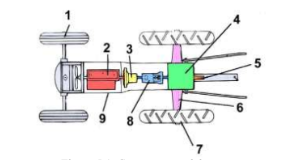
\includegraphics[width=0.8\textwidth]{./img_0009/tractor_partes.PNG}
\caption{Componentes del tractor}
\end{figure}
\end{center}
\begin{enumerate}
\item Ruedas directrices
\item Motor
\item Embrague
\item Diferencial
\item Toma de fuerza
\item Palier y reducción final
\item Ruedas motrices
\item Caja de cambios y grupo reductor
\item Bastidor
\end{enumerate}
\subsection{Trabajos que puede realizar}
\label{sec:orgda6ac81}
El tractor es una máquina que tiene diferentes aplicaciones en la agricultura y
selvicultura. Los diferentes trabajos que realiza los podemos clasificar en:
\begin{itemize}
\item \textbf{Estacionarios}.
\begin{itemize}
\item Mediante la toma de fuerza, por ejemplo accionar una bomba de riego
\item Mediante el sistema hidráulico, por ejemplo accionar un elevador de grano
\end{itemize}
\end{itemize}
\begin{center}
\begin{figure}[htbp]
\centering
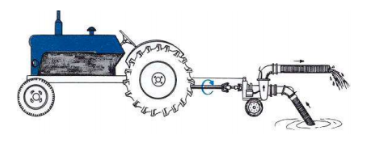
\includegraphics[width=0.8\textwidth]{./img_0009/tractor_riego.PNG}
\caption{Accionando una bomba de riego}
\end{figure}
\end{center}
\begin{itemize}
\item \textbf{De transporte}. Por ejemplo tirar un remolque
\end{itemize}
\begin{center}
\begin{figure}[htbp]
\centering
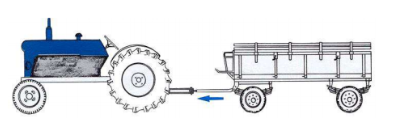
\includegraphics[width=0.8\textwidth]{./img_0009/tractor_remolque.PNG}
\caption{Transportando un remolque}
\end{figure}
\end{center}
\begin{itemize}
\item \textbf{De arrastre}. Por ejemplo tirar de un arado
\end{itemize}
\begin{center}
\begin{figure}[htbp]
\centering
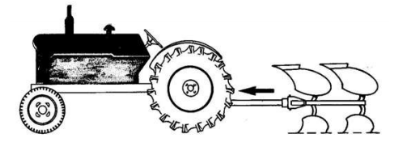
\includegraphics[width=0.8\textwidth]{./img_0009/tractor_arado.PNG}
\caption{Arrastrando un arado}
\end{figure}
\end{center}
\begin{itemize}
\item \textbf{De empuje}. Por ejemplo trabajar con una pala cargadora
\end{itemize}
\begin{center}
\begin{figure}[htbp]
\centering
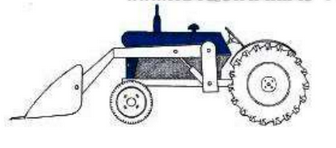
\includegraphics[width=0.8\textwidth]{./img_0009/tractor_pala.PNG}
\caption{Accionando una pala}
\end{figure}
\end{center}
\begin{itemize}
\item \textbf{Combinados}
\begin{itemize}
\item Transporte y toma de fuerza. Por ejemplo remolque accionado
\item Arrastre y toma de fuerza. Por ejemplo llevar una fresadora
\end{itemize}
\end{itemize}

Todas estas posibilidades se resumen en 4 grandes acciones que constituyen las
aplicaciones básicas del tractor:
\begin{itemize}
\item Remolcar
\item Arrastrar
\item Empujar
\item Transmitir movimiento
\end{itemize}
\subsection{Sistema de tracción del tractor}
\label{sec:orgbf0877b}

Podemos dividir el sistema de tracción de un tractor típico en las siguientes
partes:
\begin{enumerate}
\item Motor y sus componentes
\label{sec:orge563fc7}

Cilindros, bielas, cigüeñal,etc.

\item Transmisión
\label{sec:org33fb2c7}

Formada por el embrague (separa el motor de la transmisión), cambio de
velocidades y el diferencial (comunica el giro del motor a las ruedas
propulsoras).
\item Dirección
\label{sec:org363ec6a}

Se maneja a través del volante por el conductor, dirige a un lado o a otro las
ruedas.
\item Mecanismos auxiliares
\label{sec:org0ed8f28}

Frenos, sistema eléctrico,sistema de refrigeración, ruedas, sistema eléctrico,
etc.
\end{enumerate}

\subsection{El motor}
\label{sec:org988e336}

El motor proporciona la potencia y el rendimiento del tractor.  Está situado en 
la parte delantera del mismo cubierto por el capó. El combustible que utilizan
los motores de tractor es \uline{diésel}.

Visualmente podemos dividir al motor en tres partes:
\begin{itemize}
\item \textbf{Bloque motor:} es la parte central del motor donde van alojados diferentes
partes como pistones, cigüeñal, volante de inercia, etc
\item \textbf{Tapa de culata y balancines:} situado en la parte superior del bloque
motor. es la parte que canaliza los gases producidos por la combustión del carburante
\item \textbf{Cárter:} situado en la parte inferior del bloque motor. Recoge el aceite del
sistema de engrase para ser enviado a las partes móviles del motor
\end{itemize}
\subsubsection{Componentes internos del motor}
\label{sec:orgf062396}

\begin{itemize}
\item \textbf{Cilindros:} situados en el bloque del motor. Son los tubos huecos por donde
se mueven los pistones
\item \textbf{Pistones:} piezas móviles expuestas a la combustión del combustible. Realizan
un movimiento alternativo y están unidos a  las bielas para transmitir el
movimiento al cigüeñal
\item \textbf{Anillos:} situados alrededor del pistón muy próximos a la cabeza del
mismo. Su misión es que no se produzcan perdidas de gases en el cilindro
\item \textbf{Bielas:} unidas por un extremo a los pistones y por otro al
cigüeñal. Transmiten el movimiento generado por la combustión del combustible
\item \textbf{Cigüeñal:} transforma el movimiento alternativo del pistón en movimiento
rotatorio. Este movimiento rotatorio es el que hace que, además que el
tractor se desplace, funcionen los sistemas de engrase, encendido,
lubricación, toma de fuerza.
\item \textbf{Volante de inercia:} almacena la energía para que el pistón pueda volver a la
parte superior del cilindro
\item \textbf{Válvulas:} permiten la entrada y salida de gases del cilindro. Se disponen de
dos en dos (como mínimo) en el cilindro, una conectada al colector de entrada
de gases y otra al colector de salida
\item \textbf{Eje de levas o balancines:} recibe el movimiento del cigüeñal y realiza la
apertura y cierre de las válvulas
\end{itemize}
\subsubsection{Funcionamiento interno del motor. Los tiempos de funcionamiento}
\label{sec:org9e72b24}
Los tractores agrícolas y forestales funcionan mediante motores de cuatro
tiempos. Veamos los pasos de funcionamiento que sigue este tipo de motor.

\begin{enumerate}
\item \textbf{Tiempo de admisión:} entrada del aire en el cilindro. Cuando el cilindro
está lleno de aire, el pistón comienza a descender, \uline{se abre la válvula de
admisión} y la válvula de escape se encuentra \uline{cerrada}.
\item \textbf{Tiempo de compresión:} El pistón comienza su carrera ascendente y en ese
momento se \uline{cierra la válvula de admisión} produciéndose de esta manera la
\uline{compresión del aire admitido en el cilindro}
\item \textbf{Tiempo de trabajo o explosión:} inyección del combustible y combustión del
mismo. Por la elevada presión y temperatura existentes en el cilindro, se
produce la combustión del combustible que empuja al pistón. Las válvulas de
admisión y escape se encuentran cerradas.
\item \textbf{Tiempo de escape:} desalojo de los gases producidos por la combustión en la
carrera de trabajo. Debido a la inercia que tiene el cigüeñal el pistón
comienza una nueva carrera ascendente, en ese momento \uline{se abre la válvula de
escape}, y el pistón empuja los gases al colector de escape. La válvula de
admisión se encuentra cerrada y se abrirá de nuevo al finalizar la carrera
ascendente para comenzar un nuevo ciclo.
\end{enumerate}

\begin{center}
\begin{figure}[htbp]
\centering
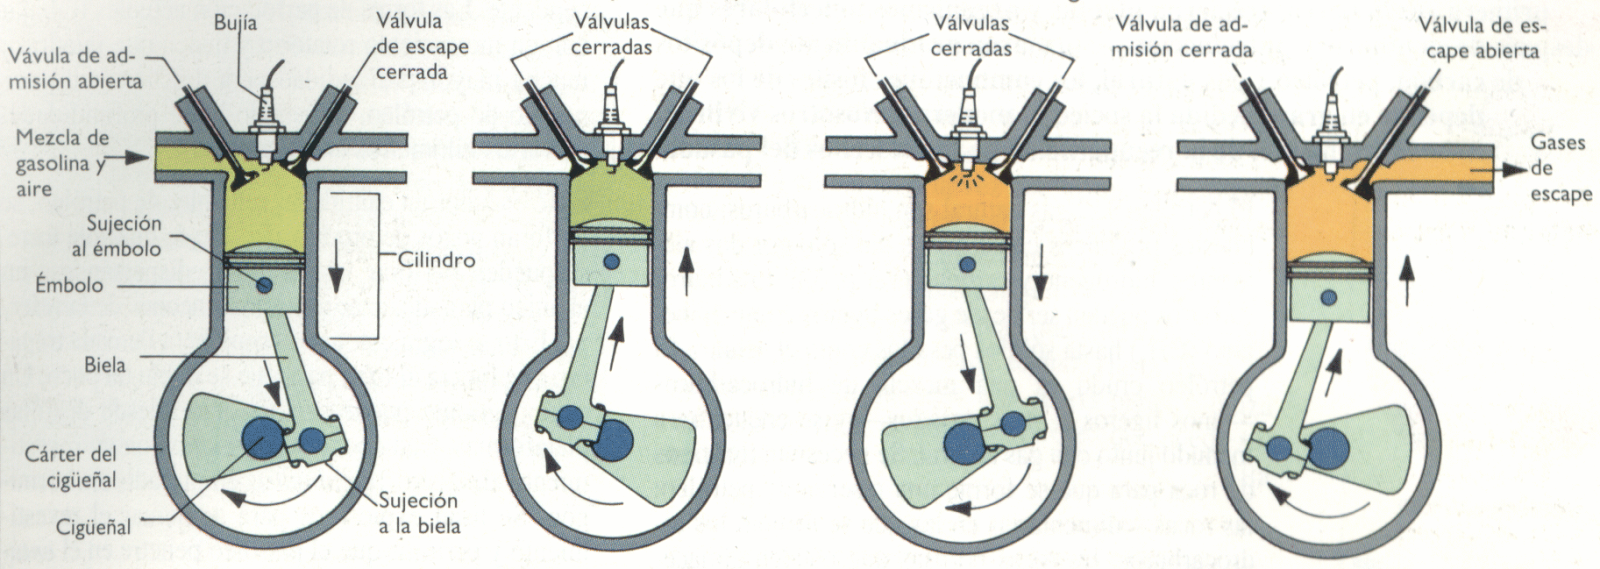
\includegraphics[width=0.65\textwidth]{./img_0009/esquema_cuatrot.png}
\caption{Esquema de distribución}
\end{figure}
\end{center}

\subsubsection{Sistema de distribución y admisión}
\label{sec:orge931ba5}
El conjunto de dispositivos necesarios para \uline{regular la entrada y salida de 
gases del cilindro} conforman la \textbf{distribución}.

\begin{center}
\begin{figure}[htbp]
\centering
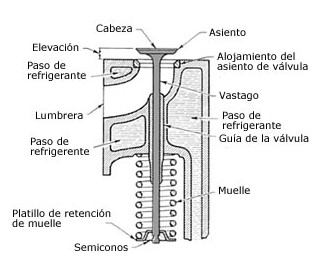
\includegraphics[width=0.65\textwidth]{./img_0009/valvulabloque.jpg}
\caption{Esquema de distribución}
\end{figure}

\begin{figure}[htbp]
\centering
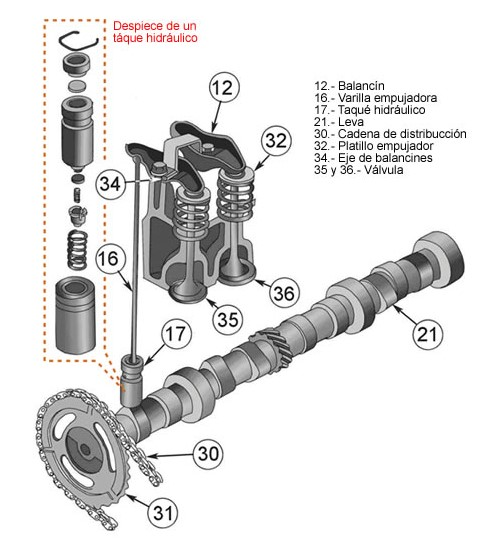
\includegraphics[width=0.65\textwidth]{./img_0009/esquema_distribucion.jpg}
\caption{}
\end{figure}
\end{center}

Los elementos principales que constituyen la distribución son los siguientes:
\begin{itemize}
\item \textbf{Válvulas:} tienen como misión abrir o cerrar los orificios de entrada de
gases al cilindro
\item \textbf{Eje de levas:} sincronizado con el cigüeñal es el encargado de que las
válvulas se abran o cierren en el momento apropiado
\item \textbf{Empujadores:} transmiten el empuje del eje de levas a los balancines
\item \textbf{Balancines:} palancas que transmiten el movimiento de las levas a las válvulas
\item \textbf{Correa o cadena de distribución :} correa que transmite el movimiento del
cigüeñal al eje de levas para que este realice su función
\end{itemize}

Estos elementos actúan en conjunto abriendo y cerrando las válvulas en los
tiempos de admisión y escape de cada cilindro. Esto se ha de realizar de forma
sincronizada con el giro del cigüeñal. 

\subsubsection{Sistema de engrase}
\label{sec:org541f0b2}
Un motor de combustión es un conjunto de piezas metálicas que se rozan un as con
otras. Este \uline{rozamiento} produce un gran \uline{desgaste y calentamiento} y puede
llevar a la rotura del motor. Para evitar esto se necesita que las piezas se
deslicen sobre una capa de aceite. El conjunto de \uline{piezas y conductos} qué hacen
que el aceite llegue a presión a todas partes se conoce por sistema de engrase o
lubricación. Este sistema consta de:
\begin{itemize}
\item \textbf{Filtro de entrada a bomba:} malla metálica que impide que entre suciedad o
partes metálicas al interior de la bomba evitando su desgaste o rotura
\item \textbf{Bomba de aceite:} recoge el aceite del cárter y lo envía a presión a las
diferentes partes del motor
\item \textbf{Filtro de aceite:} es la pieza encargada de retener las partículas más finas
que contiene el aceite y han pasado por el filtro de entrada a la bomba
\item \textbf{Control de presión:} controla que en todo momento a que presión llega el
aceite a los lugares de engrase. Puede ser un manómetro o un testigo luminoso
\end{itemize}
\subsubsection{Sistema de refrigeración}
\label{sec:orgddec6c7}
En el momento de la combustión se produce un aumento de temperatura que puede
llegar a alcanzar los 1500\textdegree{}C. Esta temperatura podría fundir muchas
piezas , por lo qué se hace necesario \uline{eliminar el exceso de calor} que se
produce, y eso se consigue mediante el sistema de refrigeración.

Existen dos sistemas de refrigeración para motores de combustión, por \uline{aire} y
por \uline{agua o líquida}. 

\begin{itemize}
\item \textbf{Refrigeración por aire:} aprovecha el aire existente alrededor del motor para
enfriarlo. son sistemas típicos de motores 2T No entraremos en detalle en
ellos ya que no son los sistemas de refrigeración que encontraremos en los
tractores agrícolas o forestales.
\item \textbf{Refrigeración liquida:} un líquido refrigerante es la encargado de enfriar el
motor. Esta  es enfriada por una corriente en el \uline{radiador} y circula a través
de  conducciones por todo el motor. Este sistema cuenta con los siguientes
componentes: 
\begin{itemize}
\item \textbf{Camisa de agua:} cámara hueca que rodea las paredes del cilindro para que
circule el líquido refrigerante
\item \textbf{Radiador:} circuito de tubos en el que se enfría el líquido refrigerante
que viene del motor antes de ser enviado de nuevo. La refrigeración del
liquido suele ser mediante una corriente de aire forzada por un ventilador
que circula a través de unas aletas que están conectadas a los tubos
\item \textbf{Manguitos:} tubos de goma que conectan el radiador con el bloque motor y
otros componentes como el depósito o la bomba
\item \textbf{Bomba de agua:} la que impulsa el líquido refrigerante por el sistema
\item \textbf{Ventilador:} fuerza la entrada de aire a través de las aletas del radiador
\item \textbf{Termostato:} es el encargado de accionar el ventilador cuando la
temperatura del agua se incrementa
\item \textbf{Termo-metro:} indica la temperatura del líquido refrigerante. Como en el
caso del aceite puede ser un indicador luminoso o de nivel
\end{itemize}
\end{itemize}
\subsubsection{Sistema de alimentación}
\label{sec:orgd9f5932}
La característica principal de los motores diésel en comparación con los
gasolina es que el combustible se inyecta en el cilindro y se quema por \uline{aumento 
de la temperatura del aire en el cilindro}. En los motores gasolina es la
\uline{bujía} la encargada de producir una chispa para que el combustible se queme,
\uline{los motores diésel no tienen bujía}.

Para que el combustible diésel llegue al cilindro ha de seguir un recorrido
desde el depósito hasta la cámara de combustión de cada cilindro alojada en la
culata del motor.

Los elementos del sistema de alimentación son los siguientes:
\begin{itemize}
\item \textbf{Deposito:} recipiente en el que se almacena el combustible para el
funcionamiento del motor
\item \textbf{Bomba de alimentación:} es la que aspira el gasóleo del deposito y la envía
con cierta presión al filtro que hay antes de la bomba de inyección
\item \textbf{Filtro de gasoil:} su misión es limpiar el gasoil antes de que llegue a la
bomba de inyección
\item \textbf{Bomba de inyección:} dosifica el combustible y lo envía a través de unas
conducciones a los inyectores en el momento adecuado para que se produzca la
combustión en el cilindro. Está sincronizada con el cigüeñal y la distribución
del motor
\item \textbf{Inyectores:} están alojados en la culata del motor. Reciben el combustible a presión desde la bomba de inyección y lo
pulveriza dentro de la cámara de combustión del cilindro
\end{itemize}
\subsubsection{Sistema de transmisión}
\label{sec:org3111a3b}
Este sistema hace que el \uline{movimiento de rotación} que se produce en el cigüeñal
pase a la \uline{caja de cambio} mediante el \textbf{embrague} y de ahí a través del
\uline{diferencial} hasta las \uline{ruedas motrices} que dan impulso al tractor.
\begin{enumerate}
\item \textbf{El embrague}
\label{sec:orgb23285d}

Es el dispositivo por el que se transmite o interrumpe el \uline{movimiento
giratorio} causado por el motor \uline{hacia la caja de cambios}

\begin{center}
\begin{center}
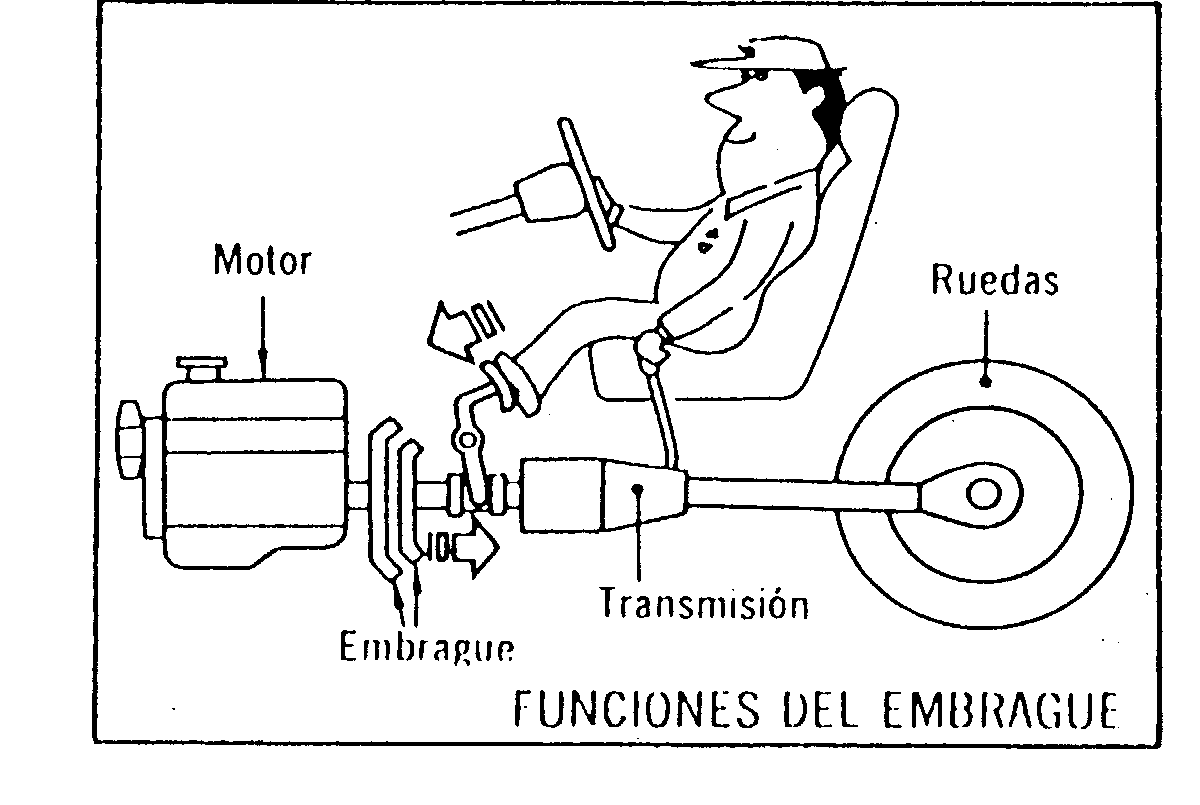
\includegraphics[width=0.65\textwidth]{./img_0009/embrague_1.png}
\end{center}
\end{center}
En esencia, un embrague consta de:
\begin{itemize}
\item \uline{Una tapa metálica o campana} que está unida al volante de inercia y que
encierra en su interior diferentes piezas
\item \uline{Un disco de embrague} que constiste en un disco metálico que lleva en su
parte pariférica dos coronas de un material \uline{altamente resistente a la fricción}.
\item \uline{Un disco opresor} del mismo tamaño del disco de embrague, con unas patillas
que actuan sobre el material resistente del disco de embrague
\item Sistema de muelles y resortes que acuan sobre los discos haciendo que estos se
\uline{aciplen y desacoplen} para transmitir el movimiento del motor a la caja de
cambios
\end{itemize}

\begin{center}
\begin{figure}[htbp]
\centering
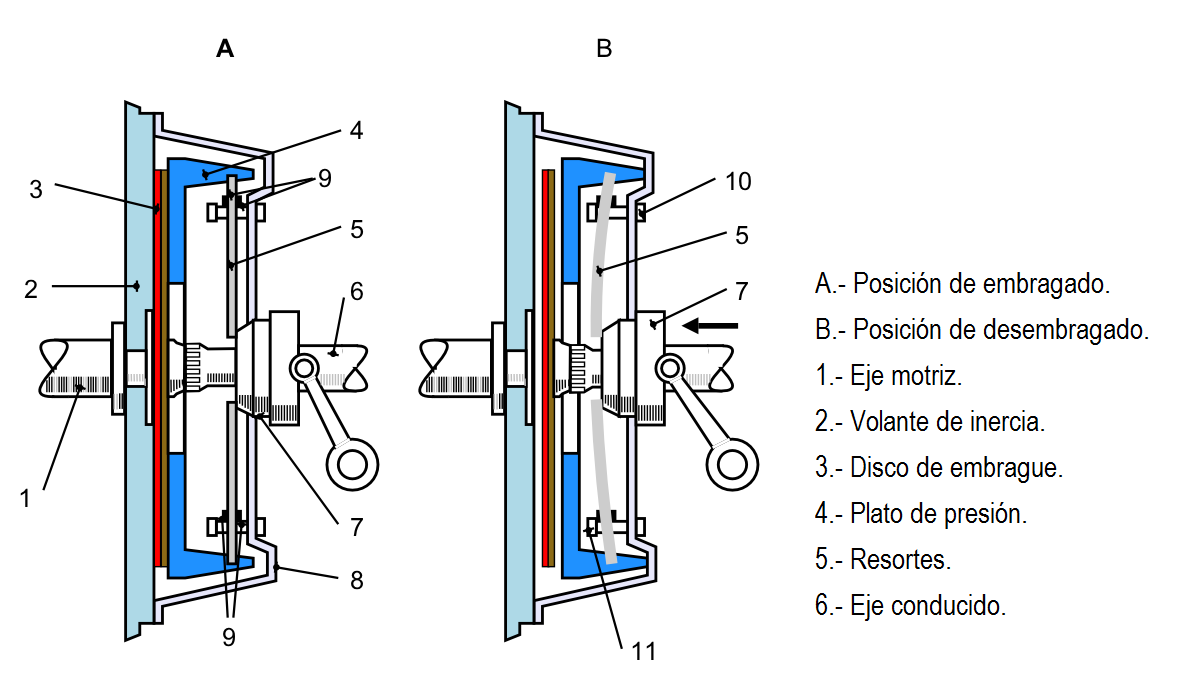
\includegraphics[width=0.65\textwidth]{./img_0009/embrague.png}
\caption{Embrague monodisco}
\end{figure}
\end{center}
\item \textbf{Caja de cambios}
\label{sec:orgf3d07cd}
\end{enumerate}


\subsection{Sistema hidraulico}
\label{sec:org8e1ad6c}
\end{document}